\documentclass{beamer}
\usetheme{default}

% Miscellaneous
\usepackage{etoolbox}

% Layout

% Graphics
\usepackage[footnotesize]{caption} % For captions
%\usepackage{caption} % For subcaptions
\usepackage{subcaption} % For subcaptions
\usepackage{tikz} % For advanced graphics functions
\usepackage{pgfplots}

% TikZ
% Two-dimensional versions
\newrobustcmd{\drawplus}[3]{;\draw (#1+#3/2,#2) -- (#1+#3/2,#2+#3); \draw (#1,#2+#3/2) -- (#1+#3,#2+#3/2);}
\newrobustcmd{\squarepath}[1]{-- ++(#1,0) -- ++(0,#1) -- ++(-#1,0) -- cycle}
% Three-dimensional versions
\newrobustcmd{\drawthreedimplus}[4]{\def\cx{#1} \def\cy{#2} \def\cz{#3} \def\s{#4} \drawthreedimplushelper}
\newrobustcmd{\drawthreedimplushelper}[6]{;\draw (\cx+\s*#1/2,\cy+\s*#2/2,\cz+\s*#3/2) -- +(\s*#4,\s*#5,\s*#6); \draw (\cx+\s*#4/2,\cy+\s*#5/2,\cz+\s*#6/2) -- +(\s*#1,\s*#2,\s*#3);}
\newrobustcmd{\threedimsquarepath}[7]{-- ++(#1*#2,#1*#3,#1*#4) -- ++(#1*#5,#1*#6,#1*#7) -- ++(-#1*#2,-#1*#3,-#1*#4) -- cycle}

\begin{document}

% % % % % % % % % % % % % % %
% Start "unnumbered" pages  %
% % % % % % % % % % % % % % %
\pagenumbering{Alph}
\pagestyle{empty}

% NOTE: Make sure to replace the \today and \shortyear macros if you are reprinting a previously published document.

%\pdfbookmark[0]{Title pages}{thetitlepagesanchor}

\title{Simulating Ocean Waves and Ships with an Octree Data Structure} % The title of the report
\author{Kristofer Krus} % Your name
\date{\today} % The date of ... (?)
%\thanks{All supporters} % In case you have someone to thank. Do not use.
\lithlogo{
\includegraphics[width=0.6\textwidth, clip=true]{./Images/lith_en_vert_col.pdf}} % The code for displaying the logo (or a replacement)
\lithcompany{Saab AB} % The company the thesis work was carried out at
\lithwork{Master thesis work} % The type of work (well master thesis work, duh)
\lithdepartment{Department of Physics, Chemistry and Biology} % The department (is there any choice here?)
\lithuniversity{Linköpings universitet} % Your university (Linköping universitet if you didn't know...)
\lithpostaladdress{SE-581 83 Linköping, Sweden} % The postal address of the university
% NOTE! Only use on of the fields lithsupervisor and lithsupervisors, comment the other out
%\lithsupervisor{Supervisor} % The supervisor
\lithsupervisors{Anders Rönnbrant (Saab AB)\\Kenneth Järrendal (Linköping Institute of Technology)} % The supervisors, separated by e.g. a comma or a double backslash
\lithexaminer{Magnus Johansson (Linköping Institute of Technology)} % The examinor of the thesis work
\lithx{A} % A or G (A for advanced, G for kandidat)
\lithyy{\shortyear} % The two last digits of the year
%\lithxxxx{} % The master thesis work number

\lithmaketitle
%\blankpage
\pdfbookmark[0]{Library page}{thelibrarypageanchor}
\thispagestyle{empty}

% NOTE: Make sure to replace the \today and \shortyear macros if you are reprinting a previously published document.

%\pdfbookmark[0]{Title pages}{thetitlepagesanchor}

%\title{Simulating Ocean Waves and Ships with an Octree Data Structure} % The title of the report
%\title{Wave Model and Watercraft Model for Simulation of Sea State} % The title of the report
%\author{Kristofer Krus} % Your name
%\date{\today} % The date of ... (?)
%\thanks{All supporters} % In case you have someone to thank. Do not use.
\ifmlogo{
\includegraphics[width=0.6\textwidth, clip=true]{./Images/lith_sigill_blk.pdf}} % The code for displaying the logo (or a replacement)
\ifmcompany{Saab AB} % The company the thesis work was carried out at
\ifmwork{Master thesis work} % The type of work (well master thesis work, duh)
\ifmdepartment{Department of Physics, Chemistry and Biology} % The department (is there any choice here?)
\ifmuniversity{Linköpings universitet} % Your university (Linköping universitet if you didn't know...)
\ifmpostaladdress{SE-581 83 Linköping, Sweden} % The postal address of the university
% NOTE! Only use on of the fields ifmsupervisor and ifmsupervisors, comment the other out
%\ifmsupervisor{Supervisor} % The supervisor
\ifmsupervisors{Anders Rönnbrant (Saab AB)\\Kenneth Järrendal (Linköping Institute of Technology)} % The supervisors, separated by e.g. a comma or a double backslash
\ifmexaminer{Magnus Johansson (Linköping Institute of Technology)} % The examinor of the thesis work
\ifmx{A} % A or G (A for advanced, G for kandidat)
\ifmyy{\shortyear} % The two last digits of the year
%\ifmxxxx{} % The master thesis work number

%\ifmmakelibrary
\begin{center}\textit{Library page}\end{center}\clearpage



\notocsection[0]{Copyright}{thecopyrightanchor}
\thispagestyle{empty} % Remove page numbering on this page

The publishers will keep this document online on the Internet -- or its possible replacement -- for a period of 25 years starting from the date of publication barring exceptional circumstances.

The online availability of the document implies permanent permission for anyone to read, to download, or to print out single copies for his/hers own use and to use it unchanged for non-commercial research and educational purpose. Subsequent transfers of copyright cannot revoke this permission. All other uses of the document are conditional upon the consent of the copyright owner. The publisher has taken technical and administrative measures to assure authenticity, security and accessibility.

According to intellectual property law the author has the right to be mentioned when his/her work is accessed as described above and to be protected against infringement.

For additional information about the Linköping University Electronic Press and its procedures for publication and for assurance of document integrity, please refer to its www home page: \url{http://www.ep.liu.se/}.

%\notocsection[0]{Abstract}{theabstractanchor}

\pdfbookmark[0]{\abstractname}{theabstractanchor}
\begin{abstract}
The problem of real-time simulation of ocean surface waves, ship movement and the coupling in between is tackled, and a number of different methods are covered and discussed, of which the finite volume method has been implemented in an attempt to solve the problem, along with the compressible Euler equations, an octree based staggered grid which allows for easy adaptive mesh refinement, the volume of fluid method and a variant of the Hyper-C advection scheme for compressible flows for advection of the phase fraction field.
    
The process of implementing the methods that were chosen proves to be tricky in many ways, and involves a large number of topics that are very advanced only by themselves, and the implementation that was implemented in \thismasterthesiswork suffered from numerous issues, including problems with keeping the interface intact and a harsh restriction on the time-step size due to the CFL condition. Improvements required to make the method sustainable are discussed, and a few suggestions on alternative approaches that are already in use for very similar purposes are also given and discussed.
    
Furthermore, a method for compensating for gain/loss of mass when solving the incompressible flow equations with an inaccurately solved pressure Poison equation is presented and discussed. A momentum conservative method for transporting the velocity field on staggered grids without introducing unnecessary smearing is also presented and implemented. A simple, physically based illumination model for sea surfaces is derived and compared to the Blinn--Phong shading model, although it is never implemented. Finally, a two-dimensional partial differential equation in the spatial domain for simulating water surface waves for mildly varying bottom topography is derived and discussed, although it is deemed to be too slow for real-time purposes and is therefore never implemented.
\end{abstract}
%%\begin{acknowledgments}
\section*{Acknowledgments}

Vi tycker alla har varit så himla goa hela den här långa och tuffa tiden i våra liv.
%\end{acknowledgments}


% % % % % % % % % % % % % % % %
% Start Roman-numbered pages  %
% % % % % % % % % % % % % % % %
\pagenumbering{roman}
\pagestyle{plain}

% Table of contents
\pdfbookmark[0]{\contentsname}{thecontentsanchor}
\tableofcontents

% List of tables
%\addtotoc{chapter}{List of Tables}
%\listoftables

% List of figures
%\addtotoc{chapter}{List of Figures}
%\listoffigures

% Notation
\nonumchapter{Notation}

\comment
{
\nonumsection{Nomenclature}
\begin{center}
% See http://en.wikipedia.org/wiki/Greek_alphabet
\begin{longtabu}{l X} % The X must be upper case
%\begin{longtabu}{|l|X|} % The X must be upper case
    %\hline
    \textbf{Notation}   & \textbf{Meaning} \\
    \hline
    \\
    \endhead
    
    $\nabla$            & The del operator, commonly used in vector algebra \\
    $\mathcal{F}$       & The non-uniform Fourier transform \\
    $\mathcal{F}^{-1}$  & The reverse non-uniform Fourier transform \\
    
    \\
    
    %alpha
    $\alpha$            & The discretized phase fraction \\
    $\alpha_i$          & The value of $\alpha$ in $C_i$ \\
    $\alpha^*$          & The non-discretized phase fraction \\
    %beta
    %gamma
    $\gamma$            & The surface tension \\
    $\gammapath$        & A path within $\phi$'s domain, connecting the vectors
                          $\vec{r}_1$ and $\vec{r}_2$ \\
    %delta
    $\Delta\vec{r}$     & Defined as $\Delta\vec{r} = \vec{r}_2 - \vec{r}_1$ \\
    %epsilon
    %zeta
    %eta
    $\eta$              & The free surface elevation \\
    $\eta_i$            & The band-pass filtered free surface elevation belining to the $i$th grid \\
    %theta
    $\theta$            & The angle between the $\vec{x}$ and $\vec{\xi}$ vectors \\
    %iota
    %kappa
    %lambda
    %mu
    $\mu$               & The (dynamic) viscosity \\
    %nu
    %xi
    $\xi,\,\vec{\xi}$   & $\vec{\xi}$ is a dimensionless vector in the frequency domain
                          and $\xi = |\vec{\xi}|$ \\
    %omicron
    %pi
    %rho
    $\rho$              & The density \\
    $\rho_0$            & The average density of the specific cell \\
    $\rho_i$            & The average density of the $i$th neighbor cell \\
    $\rho_n$            & The density in timestep $n$ \\
    %sigma
    %tau
    %upsilon
    %phi
    $\phi$              & A signed distance function, also known as level set function;
                          a scalar field \\
    $\phi'_{\vec{v}}$   & The derivative of $\phi$ in the direction of $\vec{v}$ \\
    %chi
    %psi
    %omega
    $\omega$            & The angular frequency of one wave component \\
    $\sop{\omega}$      & A scalar operator \\
    
    \\
    
    $a$                 & The thickness in number of cells of the LOD layers
                          (when all of them have the same thickness);
                          real, non-zero number for scaling of a function \\
    $a_{h_e}$           & A scale factor associated with $h_e$ \\
    $a_h,\,a_{h(\vec{r})}$      & Defined as $a_h = 1/h^2$ and $a_{h(\vec{r})} = 1/h^2(\vec{r})$
                                  respectively \\
    $a_i$               & The thickness in number of cells of LOD layer $i$ \\
    $A$                 & The wave amplitude \\
    %$\complexes$        & The set of complex numbers \\
    $c$                 & The speed of the propagation of waves;
                          a distinct level of the signed distance function $\phi$ \\
    $C$                 & The Courant number, which is basically the ratio of a cells volume that
                          is replaced in one time step because of flow through the cell walls \\
    $C_i$               & The cell with index $i$ \\
    $\sop{C}$           & A scalar operator applying a convolution filter on a function \\
    $\sop{C}_h,\,\sop{C}_{h(\vec{r})},\,\sop{C}_{h_e}$ & Versions of $\sop{C}$ associated with $h$,
                                                         $h(\vec{r})$ and $h_e$ respectively \\
    $d$                 & The number of dimensions \\
    $\opd S$            & An infinitesimal element in $S$ \\
    $\opd V$            & An infinitesimal element in $V$ \\
    $d$                 & The number of dimensions \\
    $\normvec{e}_i$     & A \idxs{base}{vector} in $\{\normvec{e}_i\}$ that is aligned
                          with the $i$th \idxs{grid}{axis} \\
    $\{\normvec{e}_i\}$ & An \idxs{orthonormal}{basis} for $\mathbb{R}^d$ \\
    $f$                 & A convolution kernel \\
    $\vec{f}$           & The external forces per unit volume \\
    $\vec{F}$           & A vector field \\
    $F_0$               & The zeroth order Hankel transform \\
    $F_i$               & The average field flux through $S_i$;
                          the $\normal_i$-component of the average value of the field on
                          the cell face $S_i$ \\
    $g$                 & The gravitational acceleration \\
    $h$                 & The water depth \\
    $h_e$               & Effective water depth \\
    $i$                 & An index; the imaginary unit \\
    $i_j$               & An index that is either 0 or 1 and corresponds to the position of the
                          child cell relative to the parent cell along $\normvec{e}_j$ \\
    $I(\alpha)$         & The interface using the discretized phase fraction \\
    $I^*(\alpha^*)$     & The interface using the non-discretized phase fraction \\
    $j$                 & An index \\
    $J_0$               & The zeroth order Bessel function of the first kind \\
    $k$                 & The wave number of one wave component; an index;
                          the number of the iterations carried out \\
    $\vec{k}$           & The wave vector of one wave component \\
    $\vop{k}$           & A vector operator \\
    $\sop{k^2}$         & A scalar operator \\
    $K$                 & A unitless convolution kernel;
                          the reverse non-uniform Fourier transform of $\fdfunc{K}$ \\
    $K^*$               & An estimate of $K$ \\
    $\fdfunc{K}$        & A frequency domain function of a unitless vector \\
    $L_c(\phi)$         & The set of all locations $\vec{r}$ where $\phi(\vec{r}) = c$ \\
    $m$                 & The mass of the fluid in $V$ \\
    $n$                 & The number of time steps taken \\
    $\normal$           & The normal of $\opd S$ \\
    $\normal_i$         & The normal of $S_i$ \\
    $N$                 & The number of surface grid points; the number of particles;
                          the number of unknowns \\
    $N_{\text{s}}$      & The total number of cells visible on the surface \\
    $N_{\text{s},i}$    & The number of cells visible on the surface belonging to LOD layer $i$ \\
    $N_{\text{t}}$      & The total number of cells used in the simulation \\
    %$\naturals$         & The set of natural numbers \\
    $O$                 & Big O notation \\
    $p$                 & The pressure \\
    $p_n$               & The pressure in time step $n$ \\
    $q$                 & A known function of $\vec{r}$ \\
    $\vec{r}$           & The location vector \\
    $\vec{r'}$          & The location of $\opd V$ and $\opd S$ respectively \\
    $r_i$               & The $\normvec{e}_i$ component of $\vec{r}$,
                          such that $r_i = \normvec{e}_i\cdot\vec{r}$ \\
    $\reals$            & The set of real numbers \\
    $S$                 & The surface of $V$ \\
    $S_i$               & The cell face to the $i$th neighbor cell;
                          the area of the cell face to the $i$th neighbor cell \\
    $t$                 & The time \\
    $T$                 & The temperature \\
    $\devstressten$     & The deviatoric stress tensor \\
    $\vec{u}$           & The velocity (vector) \\
    $\vec{u}_0$         & Tthe cell-centered velocity vector for the specific cell \\
    $\vec{u}_n$         & The velocity in time step $n$ \\
    $\vec{u}_0^*$       & A help variable \\
    $\vec{u}^*_n$       & Intermediate velocity in time step $n$ \\
    $V$                 & A control volume \\
    $V_{\epsilon,\text{t}}$     & The volume of the sphere with radius $\epsilon$,
                                  centered in $\vec{r}$ \\
    $V_{\epsilon,\text{w}}$     & The volume of the water contained within $V_{\epsilon,\text{t}}$ \\
    $V_{i,\text{t}}$    & The total volume of $C_i$ \\
    $V_{i,\text{w}}$    & The volume of the water contained within $V_{i,\text{t}}$ \\
    $w_i$               & The weight of the velocity scalar at $S_i$, used in averaging \\
    $x,\,\vec{x}$       & $\vec{x}$ is a dimensionless vector in the spatial domain
                          and $x = |\vec{x}|$ \\
    %\hline
    %\endfoot
\end{longtabu}
\end{center}
}

%\nonumsection{Technical abbreviations and acronyms}
\nonumsection{Technical acronyms}

\begin{center}
\tableoftaa
\end{center}

\nonumsection{Technical terms}

%The six ship motions in the steadily translating system are defined by (see \textit{\href{http://www.shipmotions.nl/DUT/LectureNotes/OffshoreHydromechanics.pdf}{OFFSHORE HYDROMECHANICS}}, p.~18):

\nonumsubsection{The degrees of freedom of a ship}

The six \DOF of a ship in the steadily translating system are referred to in the following manner \citep{Journee2001}:

\nonumsubsubsection{Translation}

\begin{longtabu}{l X}
    \textbf{Name} & \textbf{Along axis} \\
    \hline
    \\
    \endhead
    
	Surge & x-axis (back--front) \\
	Sway  & y-axis (starboard--port = right--left) \\
	Heave & z-axis (bottom--top) \\
\end{longtabu}

\nonumsubsubsection{Rotation}

\begin{longtabu}{l X}
    \textbf{Name} & \textbf{Around axis}\\
    \hline
    \\
    \endhead
    
    Roll  & x-axis (back--front) \\
    Pitch & y-axis (starboard--port = right--left) \\
    Yaw   & z-axis (bottom--top) \\
\end{longtabu}


% Outline of thesis
\nonumchapter{Outline of thesis}

In \partref{part:introduction}, the background of the work in this thesis work will be presented. In 
\chapref{chap:motivation}, the problem is formulated and the motivation for the work done in the thesis is presented. In \chapref{chap:requirementsanddifficulties}, some of the difficulties that are faced when solving the problem are explained. And in \chapref{chap:relatedwork}, some of the extensive amount of works that have been done to solve related problems are briefly discussed.

In \partref{part:theoreticalbackground}, the theoretical foundation on which the work that is presented in this report builds is described. In \chapref{chap:thefinitevolumemethod}, the finite volume method, which is the core of the method used in this thesis work, is described; for the Poisson equation, which arises and has to be solved in order to obtain the pressure when flow is incompressible or when the speed of sound is high, a few different solution methods are discussed; and a method that allows this equation to be only approximately solved, while still preserving mass, is presented. In \chapref{chap:octrees}, the octree, which is the framework in which the finite volume method operates in this thesis work, is described, along with the closely connected level of detail concept. In \chapref{chap:freesurfacemodeling}, a few methods used for free-surface modeling, which is necessary if the simulation is supposed to contain two or more immiscible fluids, are discussed. In \chapref{chap:advectionofproperties}, different advection schemes, which describe how scalar or vector fields are transported as the fluids move, are discussed. Finally, in \chapref{chap:methodsummary} there is a brief summary of all methods used in the thesis work, in case that was not obvious from the previous chapters.

In \partref{part:analysis} the thesis work is analyzed; \chapref{chap:results} contains some of its notable results, \chapref{chap:discussion} contains a discussion about these results and the work in general, \chapref{chap:improvements} discusses a number of improvements that would be necessary or at least highly desired if the method used in the thesis work was actually to be used in a flight simulator, and \chapref{chap:conclusions} contains some final conclusions and the most important things to remember from this report.

\partref{part:appendices} contains the attached appendices. In \appref{apdx:algorithmsanddatastructures}, a couple of the data structures used in this thesis work is described in greater detail, and an algorithm for transporting the velocity field, that preserves momentum and doesn't introduce unnecessary smearing is presented.

In \appref{apdx:illumination_model_derivation}, a simple, physically based illumination model for the rendering of water surfaces is derived and compared to the Blinn--Phong shading model. While the Blinn--Phong shading model is at least empirically based, while the illumination model presented here is purely theoretical, it is concluded that the shape of the specular highlights are very similar between the two models.

In \appref{apdx:pde_derivation}, a two-dimensional partial differential equation in the spatial domain, describing the time evolution of surface waves for intermediate, mildly varying water depths is presented. Although the method would be capable of running with the time complexity $O(N)$ per frame, it is still deemed to be too slow to be used in real-time simulations of water waves, and its behavior is unknown.


\part{Introduction}

\chapter{Motivation}

\chapter{Difficulties}

\begin{itemize}
    \item Wave dispersion
    \item Different depths gives different speeds
    \item The water should interact with moving objects
\end{itemize}

\chapter{Earlier approaches}

\section{Twodimensional methods}

\subsection{Twodimensional PDEs for shallow water}

\subsection{Spectral methods}

\begin{itemize}
    \item Reference 1: \textit{\href{http://web1.see.asso.fr/ocoss2010/Session_4/20100531111216_Monnier_OCOSS2010-Paper_MERCUDA_item_2.pdf}{Real time modelling of multispectral ocean scenes}}
    \item Reference 2: \textit{GPU-based simulation of Radar sea clutter}
\end{itemize}

\section{Threedimensional methods}

\subsection{Particles}

\subsubsection{Screen Space Meshes}

\begin{itemize}
    \item Reference: \textit{\href{http://www.matthiasmueller.info/publications/screenSpaceMeshes.pdf}{Screen Space Meshes}}
\end{itemize}

\subsection{Marker-and-Cell method (MAC)}

\begin{itemize}
    \item Reference: \textit{Numerical calculation of time-dependent viscous incompressible flow of fluid with a free surface}
    \item Described in: \textit{\href{http://people.sc.fsu.edu/~jburkardt/pdf/fluid_flow_for_the_rest_of_us.pdf}{Fluid Flow for the Rest of Us: Tutorial of the Marker and Cell Method in Computer Graphics}}
\end{itemize}

\subsection{Boundary element method}

\subsection{Finite element method}

\subsection{Finite volume method with tall cells}

\subsection{Finite volume method with octrees}

%This is the method I have choosen to use for my work, with the main reference \cite{Harlow65b}
This is the method I have choosen to use for my work, with the main reference \citealp{Losasso2004} and \citep{Popinet2003}.

\begin{itemize}
    \item Reference 1: \textit{\href{http://gfs.sourceforge.net/gerris.pdf}{Gerris: a tree-based adaptive solver for the incompressible Euler equations in complex geometries}}
    \item Reference 2: \textit{\href{http://physbam.stanford.edu/~fedkiw/papers/stanford2004-02.pdf}{Simulating Water and Smoke with an Octree Data Structure}}
\end{itemize}

\section{Twodimensional and threedimensional hybrid methods}

\section{Body (15 min)}

\begin{frame}
\frametitle{}
\end{frame}

\subsection{Related work}

\subsection{Theory (10 min)}

\subsubsection{Finite Volume Method (FVM)}
\begin{frame}
\frametitle{Finite Volume Method (FVM)}
\end{frame}

\subsubsection{Navier--Stokes equations}
\begin{frame}
\frametitle{Navier--Stokes equations}
\end{frame}

\chapter{Octrees}

An \octree is a tree \idxs{data}{structure} in which each \idxs{internal}{node} has exactly eight \idxse{child}{node}{children}. Octrees are often used to represent \idxs{three-dimensional}{data}, for which each node corresponds to a \cube in \idxs{three-dimensional}{space}, and where each of those cubes that corresponds to a \idxs{parent}{node} is subdivided into eight smaller cubes with half the side, corresponding to the children of the node. Octrees are especially usefull when the data that needs to be repersented has different requirements for the \LOD in different parts of space. They are a variant of \quadtrees in which each internal node has four children and often are used to represent \idxs{two-dimensional}{data}.

In this report, an octree is going to be considered to be a spatial data structure, and so in the text it will be used interchangeably with the cube that corresponds to the \idxs{root}{node} of the octree.

\begin{figure}
    \centering
    \subcaptionbox{\label{fig:quadtree}}[.415\textwidth]{
        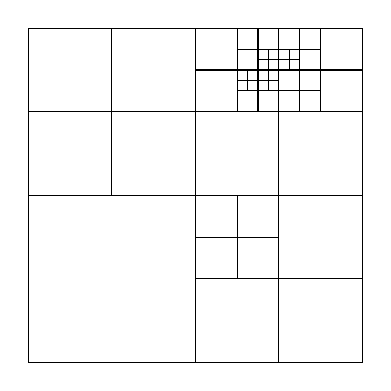
\begin{tikzpicture}[x={(.35\textwidth,0)},y={(0,.35\textwidth)}]
            % Three-dimensional versions
            \newrobustcmd{\drawthreedplus}[4]{\def\cx{#1} \def\cy{#2} \def\cz{#3} \def\s{#4} \drawthreedplushelper}
            \newrobustcmd{\drawthreedplushelper}[6]{;\draw (\cx+\s*#1/2,\cy+\s*#2/2,\cz+\s*#3/2) -- +(\s*#4,\s*#5,\s*#6); \draw (\cx+\s*#4/2,\cy+\s*#5/2,\cz+\s*#6/2) -- +(\s*#1,\s*#2,\s*#3);}
            \newrobustcmd{\threedrectpath}[7]{-- ++(#1*#2,#1*#3,#1*#4) -- ++(#1*#5,#1*#6,#1*#7) -- ++(-#1*#2,-#1*#3,-#1*#4) -- cycle}
            
            % Front side
            \draw (0,0,1) \threedrectpath{1} {1}{0}{0} {0}{1}{0};
            % Level 1
            \drawthreedplus{0}{0}{1} {1} {1}{0}{0} {0}{1}{0}
            % Level 2
            \drawthreedplus{1/2}{1/2}{1} {1/2} {1}{0}{0} {0}{1}{0}
            \drawthreedplus{1/2}{0/2}{1} {1/2} {1}{0}{0} {0}{1}{0}
            \drawthreedplus{0/2}{1/2}{1} {1/2} {1}{0}{0} {0}{1}{0}
            % Level 3
            \drawthreedplus{2/4}{3/4}{1} {1/4} {1}{0}{0} {0}{1}{0}
            \drawthreedplus{3/4}{3/4}{1} {1/4} {1}{0}{0} {0}{1}{0}
            \drawthreedplus{2/4}{1/4}{1} {1/4} {1}{0}{0} {0}{1}{0}
            % Level 4
            \drawthreedplus{5/8}{7/8}{1} {1/8} {1}{0}{0} {0}{1}{0}
            \drawthreedplus{6/8}{7/8}{1} {1/8} {1}{0}{0} {0}{1}{0}
            \drawthreedplus{5/8}{6/8}{1} {1/8} {1}{0}{0} {0}{1}{0}
            \drawthreedplus{6/8}{6/8}{1} {1/8} {1}{0}{0} {0}{1}{0}
            % Level 5
            \drawthreedplus{12/16}{14/16}{1} {1/16} {1}{0}{0} {0}{1}{0}
            \drawthreedplus{11/16}{14/16}{1} {1/16} {1}{0}{0} {0}{1}{0}
            \drawthreedplus{11/16}{13/16}{1} {1/16} {1}{0}{0} {0}{1}{0}
            \drawthreedplus{10/16}{13/16}{1} {1/16} {1}{0}{0} {0}{1}{0}
        \end{tikzpicture}
    }
    \subcaptionbox{\label{fig:octree}}[.575\textwidth]{
        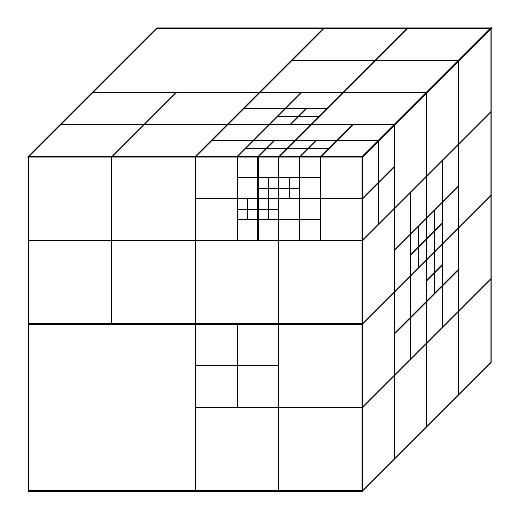
\begin{tikzpicture}[x={(.35\textwidth,0)},y={(0,.35\textwidth)},z={(-.385*.35\textwidth,-.385*.35\textwidth)}]
            % Two-dimensional versions
            %\newrobustcmd{\drawplus}[3]{;\draw (#1+#3/2,#2) -- (#1+#3/2,#2+#3); \draw (#1,#2+#3/2) -- (#1+#3,#2+#3/2);}
            %\newrobustcmd{\rectanglepath}[1]{-- ++(#1,0) -- ++(0,#1) -- ++(-#1,0) -- cycle}
            
            % Three-dimensional versions
            \newrobustcmd{\drawthreedplus}[4]{\def\cx{#1} \def\cy{#2} \def\cz{#3} \def\s{#4} \drawthreedplushelper}
            \newrobustcmd{\drawthreedplushelper}[6]{;\draw (\cx+\s*#1/2,\cy+\s*#2/2,\cz+\s*#3/2) -- +(\s*#4,\s*#5,\s*#6); \draw (\cx+\s*#4/2,\cy+\s*#5/2,\cz+\s*#6/2) -- +(\s*#1,\s*#2,\s*#3);}
            \newrobustcmd{\threedrectpath}[7]{-- ++(#1*#2,#1*#3,#1*#4) -- ++(#1*#5,#1*#6,#1*#7) -- ++(-#1*#2,-#1*#3,-#1*#4) -- cycle}
            
            % Front side
            \draw (0,0,1) \threedrectpath{1} {1}{0}{0} {0}{1}{0};
            % Level 1
            \drawthreedplus{0}{0}{1} {1} {1}{0}{0} {0}{1}{0}
            % Level 2
            \drawthreedplus{1/2}{1/2}{1} {1/2} {1}{0}{0} {0}{1}{0}
            \drawthreedplus{1/2}{0/2}{1} {1/2} {1}{0}{0} {0}{1}{0}
            \drawthreedplus{0/2}{1/2}{1} {1/2} {1}{0}{0} {0}{1}{0}
            % Level 3
            \drawthreedplus{2/4}{3/4}{1} {1/4} {1}{0}{0} {0}{1}{0}
            \drawthreedplus{3/4}{3/4}{1} {1/4} {1}{0}{0} {0}{1}{0}
            \drawthreedplus{2/4}{1/4}{1} {1/4} {1}{0}{0} {0}{1}{0}
            % Level 4
            \drawthreedplus{5/8}{7/8}{1} {1/8} {1}{0}{0} {0}{1}{0}
            \drawthreedplus{6/8}{7/8}{1} {1/8} {1}{0}{0} {0}{1}{0}
            \drawthreedplus{5/8}{6/8}{1} {1/8} {1}{0}{0} {0}{1}{0}
            \drawthreedplus{6/8}{6/8}{1} {1/8} {1}{0}{0} {0}{1}{0}
            % Level 5
            \drawthreedplus{12/16}{14/16}{1} {1/16} {1}{0}{0} {0}{1}{0}
            \drawthreedplus{11/16}{14/16}{1} {1/16} {1}{0}{0} {0}{1}{0}
            \drawthreedplus{11/16}{13/16}{1} {1/16} {1}{0}{0} {0}{1}{0}
            \drawthreedplus{10/16}{13/16}{1} {1/16} {1}{0}{0} {0}{1}{0}
            
            % Top side
            \draw (0,1,0) \threedrectpath{1} {1}{0}{0} {0}{0}{1};
            % Level 1
            \drawthreedplus{0}{1}{0} {1} {1}{0}{0} {0}{0}{1}
            % Level 2
            \drawthreedplus{0/2}{1}{1/2} {1/2} {1}{0}{0} {0}{0}{1}
            \drawthreedplus{1/2}{1}{1/2} {1/2} {1}{0}{0} {0}{0}{1}
            \drawthreedplus{1/2}{1}{0/2} {1/2} {1}{0}{0} {0}{0}{1}
            % Level 3
            \drawthreedplus{2/4}{1}{3/4} {1/4} {1}{0}{0} {0}{0}{1}
            \drawthreedplus{3/4}{1}{3/4} {1/4} {1}{0}{0} {0}{0}{1}
            \drawthreedplus{2/4}{1}{2/4} {1/4} {1}{0}{0} {0}{0}{1}
            % Level 4
            \drawthreedplus{5/8}{1}{7/8} {1/8} {1}{0}{0} {0}{0}{1}
            \drawthreedplus{6/8}{1}{7/8} {1/8} {1}{0}{0} {0}{0}{1}
            \drawthreedplus{5/8}{1}{5/8} {1/8} {1}{0}{0} {0}{0}{1}
            
            % Right side
            \draw (1,0,0) \threedrectpath{1} {0}{1}{0} {0}{0}{1};
            % Level 1
            \drawthreedplus{1}{0}{0} {1} {0}{1}{0} {0}{0}{1}
            % Level 2
            \drawthreedplus{1}{1/2}{1/2} {1/2} {0}{1}{0} {0}{0}{1}
            \drawthreedplus{1}{0/2}{1/2} {1/2} {0}{1}{0} {0}{0}{1}
            \drawthreedplus{1}{1/2}{0/2} {1/2} {0}{1}{0} {0}{0}{1}
            \drawthreedplus{1}{0/2}{0/2} {1/2} {0}{1}{0} {0}{0}{1}
            % Level 3
            \drawthreedplus{1}{3/4}{3/4} {1/4} {0}{1}{0} {0}{0}{1}
            \drawthreedplus{1}{2/4}{2/4} {1/4} {0}{1}{0} {0}{0}{1}
            \drawthreedplus{1}{2/4}{1/4} {1/4} {0}{1}{0} {0}{0}{1}
            \drawthreedplus{1}{1/4}{2/4} {1/4} {0}{1}{0} {0}{0}{1}
            \drawthreedplus{1}{1/4}{1/4} {1/4} {0}{1}{0} {0}{0}{1}
            % Level 4
            \drawthreedplus{1}{3/8}{3/8} {1/8} {0}{1}{0} {0}{0}{1}
            \drawthreedplus{1}{4/8}{3/8} {1/8} {0}{1}{0} {0}{0}{1}
            \drawthreedplus{1}{4/8}{4/8} {1/8} {0}{1}{0} {0}{0}{1}
        \end{tikzpicture}
    }
    \caption{\subrefp{fig:quadtree} A \quadtree used to partition twodimensional space. \subrefp{fig:octree} An \octree used to partition three-dimensional space. Note that an octree is essentially the same as a quadtree but is extended from two to three dimensions. In this illustration, only half of the surface of the octree is visible.}
    \label{fig:quadtree_and_octree}
\end{figure}

%\pgfmathsetseed{1}
%\foreach \col in {black,red,green,blue}
%{
%    \begin{tikzpicture}[x=10pt,y=10pt,ultra thick,baseline,line cap=round]
%    \coordinate (current point) at (0,0);
%    \coordinate (old velocity) at (0,0);
%    \coordinate (new velocity) at (rand,rand);
%    \foreach \i in {0,1,...,100}
%    {
%        \draw[\col!\i] (current point)
%        .. controls ++([scale=-1]old velocity) and
%        ++(new velocity) .. ++(rand,rand)
%        coordinate (current point);
%        \coordinate (old velocity) at (new velocity);
%        \coordinate (new velocity) at (rand,rand);
%    }
%    \end{tikzpicture}
%}

\section{Varying level of detail}

In \thisprojectwork, an octree has been used to partition the \idxs{computational}{domain} (the space in which the simulation will be performed) into the \cells required by the \FVM. Since only the \surface of the water is visible in the \simulation, the \idxsp{surface}{cell}{s} have been given a high \LOD; the \LOD then decreases at the water depth increases, staying a few \idxse{layer of}{cells}{layers of cells} a time on each \LOD, forming a \idxs{LOD}{layer} (a layer consisting of cells which all have the same \LOD, surrounded by cells with other \LODs).

Ideally, although not implemented in \thisprojectwork because of \itslimitedtime, the surface will have a higher \LOD where the \idxsp{surface}{detail}{s} are more important to the simulation, such as close to the \camera where they are more easily seen, and a lower \LOD far away from the camera where the cells take up little \idxse{screen}{space}{space on the screen}, or where they are out of the \FOV.

The total number of cells $N_{\text{t}}$ used in the simulationcan can be \approximated by an expression containing the thicknesses of the different LOD layers and the number of cells visible at the surface that belong to each \LOD accoring to

\begin{equation} \label{eq:number_of_cells_total_sum}
N_{\text{t}} \,=\, \sum_{i\,=\,0}^\infty N_{\text{s},i}\sum_{j\,=\,i}^\infty d_j\cdot 4^{-(j-i)},
\end{equation}

where $N_{\text{s},i}$ is the number of cells visible on the surface belonging to LOD layer $i$, and $d_j$ is the thickness in number of cells of LOD layer $j$, where LOD layer $0$ corresponds to the highest \LOD and an increasing LOD layer index corresponds to a lower \LOD. Different LOD layers can have different thickness; if this is the case, it will also be reflected in the simulation and waves with different wavelengths will be simulated with different \accuracy. In \thisprojectwork, all LOD layers have been given the same thickness, $d$. \eqref{eq:number_of_cells_total_sum} therefore turns into

\begin{equation} \label{eq:number_of_cells_total}
N_{\text{t}} \,=\, d\sum_{i\,=\,0}^\infty N_{\text{s},i}\sum_{k\,=\,0}^\infty 4^{-k} \,=\, d\,N_{\text{s}}\,\frac{1}{1-4^{-1}} \,=\, \frac{4}{3}\,d\,N_{\text{s}},
\end{equation}

where $k = j-i$ and $N_{\text{s}}$ is the total number of cells visible on the surface. We can therefore in this case conclude that

\begin{equation} \label{eq:number_of_cells_total_ordo}
N_{\text{t}} \,=\, O(N_{\text{s}}).
\end{equation}

Hence, the \idx{time step} for updating the \idxs{fluid}{flow} is roughly porportional to the number of \idxsp{surface}{cell}{s} $N_{\text{s}}$, but the simulation still catches all motion under the surface, with decaying \accuracy at increasing \idxsp{water}{depth}{s}.

\section{The differentiating problem}

\subsection{Perturbed cell interfaces method}

\subsection{Distributed velocities method}

\section{Multilevel acceleration}

\section{Spurious wave reflections at level transitions}

\subsubsection{Free-Surface Modeling (FSM)}
\begin{frame}
\frametitle{Free-Surface Modeling (FSM)}
\end{frame}

\subsubsection{Fluid--Structure Interaction (FSI)}
\begin{frame}
\frametitle{Fluid--Structure Interaction (FSI)}
\end{frame}

\subsubsection{Wave generation}
\begin{frame}
\frametitle{Wave generation}
\end{frame}

\subsubsection{Rendering}
\begin{frame}
\frametitle{Rendering}
\end{frame}


\subsection{Analysis}
\begin{frame}
\frametitle{Analysis}
\end{frame}

\subsubsection{Results}
\begin{frame}
\frametitle{Results}
\end{frame}

\subsubsection{Discussion}
\begin{frame}
\frametitle{Discussion}
\end{frame}

\subsubsection{Improvements}
\begin{frame}
\frametitle{Improvements}
\end{frame}

\begin{frame}
\frametitle{}
\end{frame}





\end{document}
